\section*{Chapter 8}

\subsection*{8.17 Consider the BANK ER schema in Figure 7.21, and suppose that it is necessary to keep track of different types of ACCOUNTS (SAVINGS\_ACCTS, CHECKING\_ACCTS, ...) and LOANS (CAR\_LOANS, HOME\_LOANS, ...). Suppose that it is also desirable to keep track of each ACCOUNT's TRANSACTIONS (deposits, withdrawals, checks, ...) and each LOAN's PAYMENTS; both of these include the amount, date, and time. Modify the BANK schema, using ER and EER concepts of specialization and generalization. State any assumptions you make about the additional requirements.}

\begin{center}
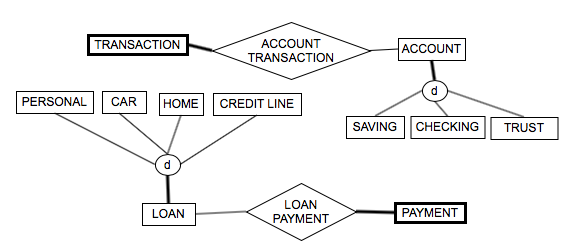
\includegraphics[width=15cm]{images/8-17.png}
\end{center}